%La distribución salarial por edad complementa esta evidencia. 
La Figura \ref{fig:edad} muestra una mayor concentración de los salarios juveniles cerca del mínimo y una menor participación de los jóvenes en los ingresos superiores al mínimo. Entre quienes reportan trabajar más de 40 horas, el 81\% de los menores de 25 años recibe hasta 1,25 mínimos, frente al 60\% de los de 25 años o más. Mientras tanto, solo el 4\% de los menores de 25 años gana dos mínimos o más, frente al 20\% de los de 25 años o más.

\begin{figure}[H]
\centering
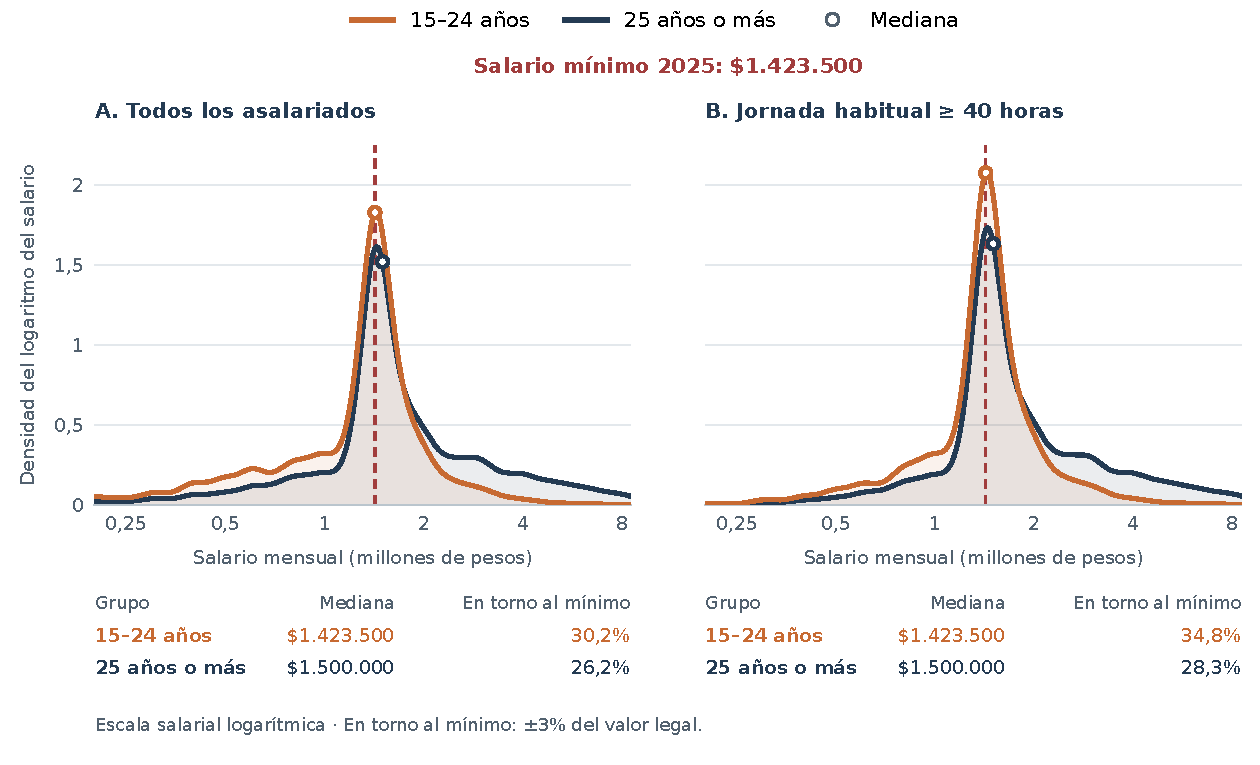
\includegraphics[width=\textwidth]{distribucion_salarios_edad_2025.pdf}
\caption{Distribución del salario mensual por edad, 2025}
\label{fig:edad}
\fuente{Fuente: DANE, GEIH 2025. Cálculos del Centro Javeriano de Competitividad \citep{orozcoGEIH}.}
\end{figure}


%La cercanía entre el piso y los salarios de otros grupos ayuda a describir la compresión salarial, entendida como una reducción de las distancias entre remuneraciones. Para medir su evolución se necesitan comparaciones de trabajadores equivalentes a lo largo del tiempo. Esta distribución de un solo año no demuestra que esas distancias hayan disminuido.

%La comparación comprende asalariados con ingreso positivo, sin distinguir formalidad, y deja fuera a quienes no consiguieron empleo. Las diferencias por edad también pueden reflejar experiencia, educación, ocupación y sector. Por eso, la concentración observada orienta el análisis de los ingresos juveniles, pero no identifica por sí sola el efecto del mínimo sobre su contratación.
